\documentclass[pdflatex,sn-mathphys-num]{sn-jnl}% Math and Physical Sciences Numbered Reference Style
\usepackage{iftex}
\ifXeTeX
  % XeLaTeX/Tectonic: Latin Modern = the template's Computer Modern look, with Vietnamese diacritics for author names.
  \usepackage{fontspec}
  \setmainfont{lmroman10}[Extension=.otf, UprightFont=*-regular, BoldFont=*-bold,
    ItalicFont=*-italic, BoldItalicFont=*-bolditalic]
\else
  \usepackage[T5,T1]{fontenc}
  \usepackage[utf8]{inputenc}
\fi
\usepackage{graphicx}%
\usepackage{multirow}%
\usepackage{amsmath,amssymb,amsfonts}%
\usepackage{xcolor}%
\usepackage{textcomp}%
\usepackage{booktabs}%
\usepackage{array}%
\usepackage{tikz}
\usetikzlibrary{arrows.meta,positioning,fit}

\raggedbottom

\begin{document}

\title[Where Should Resolution Be Preserved?]{Where Should Resolution Be Preserved? Slicing, Tiled Inference and Heterogeneous Box Fusion for Small Bird Detection}

% Vietnamese order: family name (\sur) first, then given names (\fnm).
\author[1]{\sur{Vũ} \fnm{Quốc Đạt}}\email{qd130506@gmail.com}
\author[1]{\sur{Nguyễn} \fnm{Gia Phúc}}\email{phucoik@gmail.com}
\author*[1]{\sur{Ngô} \fnm{Ngọc Trường Sơn}}\email{truongsonks2006@gmail.com}

\affil*[1]{\orgname{FPT University}, \orgaddress{\city{Da Nang}, \country{Vietnam}}}

\abstract{Birds in the MVA 2023 Small Object Detection Challenge for Spotting Birds (SOD4SB) occupy a median of 16 pixels
in 3840$\times$2160 frames, which makes every choice that touches image resolution decisive. We study where
resolution should be preserved: during training, during inference, or in the fusion of complementary detectors.
Starting from a YOLOv8-M detector pretrained on Drone2021 and fine-tuned on native-resolution crops, we compare
three training-time data strategies (colour augmentation, copy-paste and exhaustive tile sampling, ``slicing''),
two inference-time strategies (horizontal-flip test-time augmentation and SAHI tiled inference), several box
merging rules, and a heterogeneous ensemble with a GFL ResNet-50 FPN detector. Slicing gives the largest single
gain (70.2\% to 79.3\% AP50), whereas SAHI \emph{reduces} accuracy (79.3\% to 67.5\%) when full frames are already
processed without downscaling; we trace the loss to scale mismatch, tile-border truncation and over-confident
empty tiles, and show that correcting them recovers but does not exceed plain inference. Weighted boxes fusion
(WBF) of flipped and unflipped predictions reaches 81.0\%, and a single WBF over YOLO, flipped YOLO and GFL
reaches 84.5\% AP50, 45.8\% AP75 and 53.4\% AR100 on the validation split. A scale-wise analysis explains the gain:
YOLO is stronger on 8--16 px birds and GFL on 32--64 px birds. Merging rules and ensemble choices are checked on
held-out halves of the validation set, and the code and results are publicly available.}

\keywords{small object detection, bird detection, slicing, test-time augmentation, weighted boxes fusion, ensemble}

\maketitle


%=====================================================================
\section{Introduction}
%=====================================================================
Detecting birds in high-resolution video is needed for drone safety, airport bird-strike prevention and wind
farm monitoring~\cite{fujii2021distant,sun2022airbirds,yoshihashi2017windfarm}. The SOD4SB
challenge~\cite{kondo2023sod4sb} formalises this task: 4K frames, a single \emph{bird} class, and objects that
are mostly smaller than 32 pixels. At this scale the detector sees only a few pixels of texture, birds are
easily confused with leaves, wires and compression noise, and a one-pixel localisation error changes the
intersection over union (IoU) noticeably.

Two families of remedies are common in small object detection. \emph{Training-time} remedies change the data the
detector learns from, for example cropping high-resolution images instead of shrinking them, or pasting extra
objects~\cite{ghiasi2021copypaste}. \emph{Inference-time} remedies change how predictions are produced, for example
slicing-aided hyper inference (SAHI)~\cite{akyon2022sahi}, test-time augmentation (TTA) and model
ensembling~\cite{solovyev2021wbf,hou2023ensemble}. These remedies are often combined in challenge solutions,
but it is rarely shown which of them are complementary and which are redundant under a given pipeline.

This paper answers that question with controlled ablations on SOD4SB, and Section~\ref{sec:process} reports how
the study was carried out on a single laptop GPU, including the problems met on the way. Our main contributions are:
\begin{itemize}
\item We compare colour augmentation, copy-paste and exhaustive tile sampling (slicing) on the same
YOLOv8-M~\cite{jocher2023yolov8} initialisation and schedule, and find that only slicing helps (+9.1 AP50).
\item We show that SAHI degrades a detector that already processes full frames at native resolution, identify
three causes (scale mismatch, truncated boxes at tile borders, over-confident empty tiles), and quantify how much
each correction recovers.
\item We show that a single weighted boxes fusion of a slicing-trained YOLOv8-M, its flipped view and a GFL
detector~\cite{li2020gfl} raises AP50 from 79.3\% to 84.5\%, and explain the gain with a scale-wise analysis in
which the two architectures are strong on different bird sizes.
\item We report an evaluation protocol that guards against selection bias (held-out halves of the validation
set) and release code, configurations and per-image results.
\end{itemize}

%=====================================================================
\section{Related Work}
%=====================================================================
Bird datasets include wind-farm time-lapse images~\cite{yoshihashi2017windfarm}, airport surveillance
(AirBirds)~\cite{sun2022airbirds} and drone-mounted cameras (Drone2021)~\cite{fujii2021distant}, which also
serves as a pretraining source in SOD4SB~\cite{kondo2023sod4sb}. General detectors such as Faster
R-CNN~\cite{ren2015faster}, Cascade R-CNN~\cite{cai2018cascade}, CenterNet~\cite{zhou2019objects}, GFL~\cite{li2020gfl}
and VarifocalNet~\cite{zhang2021varifocalnet} were designed on COCO~\cite{lin2014coco}, where tiny objects are
rare. Tiny-object work therefore revisits matching and metrics, e.g. the normalised Wasserstein
distance~\cite{wang2021nwd}, universal-scale benchmarks~\cite{shinya2022usb} and scale-wise evaluation~\cite{shinya2023bandre}.

SAHI~\cite{akyon2022sahi} fine-tunes on slices and, at test time, predicts on overlapping tiles that are
upsampled to the network input, merging the results with the full-image prediction. Its premise is that the
full image would otherwise be downscaled. We revisit this premise for a pipeline that never downscales.

Flip TTA and multi-model ensembles are standard in challenges. Non-maximum suppression (NMS) keeps one box per
cluster, whereas weighted boxes fusion (WBF)~\cite{solovyev2021wbf} averages the coordinates of all members.
The SOD4SB winning solutions combined several detectors~\cite{kondo2023sod4sb,hou2023ensemble}; we isolate the
contribution of architectural diversity with a scale-wise analysis.

%=====================================================================
\section{The Proposed Method}
\label{sec:method}
%=====================================================================
\begin{figure}[t]
\centering
\resizebox{0.85\textwidth}{!}{%
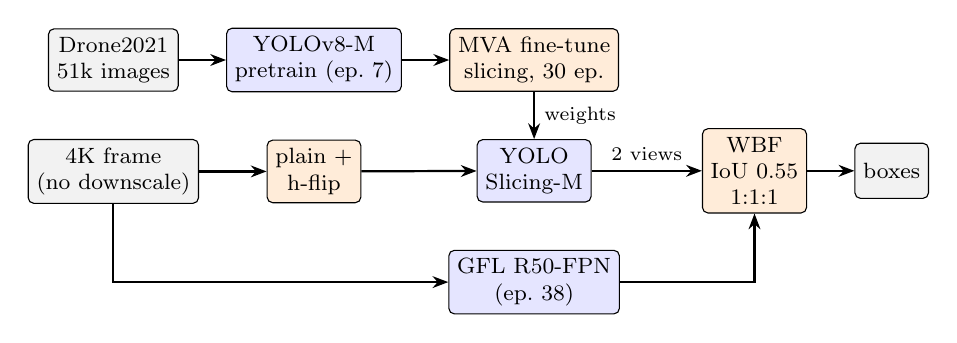
\begin{tikzpicture}[
  node distance=4mm and 6mm,
  box/.style={draw, rounded corners=2pt, align=center, font=\footnotesize, minimum height=7mm, inner sep=3pt},
  data/.style={box, fill=gray!10},
  model/.style={box, fill=blue!10},
  op/.style={box, fill=orange!15},
  arr/.style={-{Stealth[length=2mm]}, thick}]
% row 1: training chain; row 2: YOLO inference; row 3: GFL inference
\node[data] (drone) {Drone2021\\51k images};
\node[model, right=of drone] (yolo0) {YOLOv8-M\\pretrain (ep.~7)};
\node[op, right=of yolo0] (slice) {MVA fine-tune\\slicing, 30 ep.};
\node[data, below=6mm of drone] (img) {4K frame\\(no downscale)};
\node[op, below=6mm of yolo0] (flip) {plain +\\h-flip};
\node[model, below=6mm of slice] (yolo) {YOLO\\Slicing-M};
\node[model, below=6mm of yolo] (gfl) {GFL R50-FPN\\(ep.~38)};
\node[op, right=14mm of yolo] (wbf) {WBF\\IoU 0.55\\1:1:1};
\node[data, right=of wbf] (out) {boxes};
\draw[arr] (drone) -- (yolo0);
\draw[arr] (yolo0) -- (slice);
\draw[arr] (slice) -- node[right, font=\scriptsize]{weights} (yolo);
\draw[arr] (img) -- (flip);
\draw[arr] (flip) -- (yolo);
\draw[arr] (img.south) |- (gfl.west);
\draw[arr] (yolo) -- node[above, font=\scriptsize]{2 views} (wbf);
\draw[arr] (gfl.east) -| (wbf.south);
\draw[arr] (wbf) -- (out);
\end{tikzpicture}}
\caption{Final pipeline. A slicing-trained YOLOv8-M predicts on the full native-resolution frame and on its
horizontal mirror; a GFL ResNet-50 FPN predicts on the same frame. One weighted boxes fusion merges the three
sources with equal weights.}
\label{fig:pipeline}
\end{figure}

\subsection{Problem Formulation}
Let $I\in\{0,\dots,255\}^{H\times W\times 3}$ be a video frame with $H=2160$ and $W=3840$, and let
$\mathcal{G}=\{g_j\}_{j=1}^{n}$ be its annotated birds, each an axis-aligned box $g_j=(x_1,y_1,x_2,y_2)$. A detector
$f$ maps the frame to a set of scored boxes $\mathcal{B}=f(I)=\{(b_i,s_i)\}$ with $b_i\in\mathbb{R}^4$ and
$s_i\in[0,1]$. A prediction is correct at threshold $t$ if its intersection over union with an unmatched annotated
box, $\mathrm{IoU}(b,g)=|b\cap g|/|b\cup g|$, is at least $t$. Birds have a median $\sqrt{\text{area}}$ of 16 pixels,
less than 0.5\% of the frame width, so any operation that rescales $I$ changes what the detector can see.

Resolution can be preserved, or lost, at three places: in the training samples from which $f$ is learned, in the
views $v$ on which it predicts at test time, with $\mathcal{B}_v=v^{-1}\bigl(f(v(I))\bigr)$ mapped back to frame
coordinates, and in the fusion $\Phi$ of several sources. With a YOLOv8-M detector $f_Y$, a GFL detector $f_G$ and
the horizontal flip $h$, the final system is
\begin{equation}
\hat{\mathcal{B}}=\Phi\Bigl(f_Y(I),\; h^{-1}\bigl(f_Y(h(I))\bigr),\; f_G(I)\Bigr).
\label{eq:system}
\end{equation}

\subsection{Framework}
Fig.~\ref{fig:pipeline} summarises the final system. Each component was retained only if it improved AP50 in a
controlled ablation; components that were tried and rejected (colour augmentation, copy-paste, SAHI) are analysed
in Section~\ref{sec:experiments}.

\subsubsection{Detectors and Pretraining}
\textbf{YOLOv8-M.} We use the Ultralytics YOLOv8-M architecture~\cite{jocher2023yolov8} with one class. It is
trained from random initialisation on Drone2021 for 10 epochs; the epoch-7 checkpoint, which has the highest
Drone2021 validation AP50 (44.6\%), initialises every MVA branch. Each training sample is a native-resolution 1280$\times$736 crop: no
resizing is applied, so a 12-pixel bird remains 12 pixels.

\textbf{GFL.} The second detector is Generalized Focal Loss (GFL)~\cite{li2020gfl} with a ResNet-50~\cite{he2016resnet}
and FPN~\cite{lin2017fpn}, implemented with UniverseNet~\cite{shinya2022usb}. It is trained from random
initialisation on Drone2021 for 6 epochs and then on MVA, with input 2560$\times$1440 (a 2/3 downscale of the 4K frame),
batch size one with gradient accumulation over eight images, and per-image batch normalisation, which is used
identically in training and inference. Of the 50 MVA epochs we use epoch 38, the one with the highest validation
AP50 (Section~\ref{sec:metrics}).

\subsubsection{Training-Time Data Strategies}
All YOLO branches share the same initial weights, optimiser, schedule, batch size and a common augmentation
(horizontal flip with $p=0.5$ and brightness scaling in $[0.8,1.2]$). They differ only in how crops are produced:
\begin{itemize}
\item \textbf{Baseline:} one bird-centred native crop per image per epoch.
\item \textbf{Colour augmentation:} the baseline plus, with $p=0.8$, a hue shift of $\pm5$, saturation and gamma
scaling in $[0.8,1.2]$.
\item \textbf{Copy-paste:} the baseline plus, with $p=0.3$, up to three bird patches (from a bank of 24{,}485
training patches) pasted at random positions~\cite{ghiasi2021copypaste}.
\item \textbf{Slicing:} every tile of a 25\%-overlap grid of 1280$\times$736 windows that contains a bird, plus one
bird-free tile per image, is used in every epoch. This yields 31{,}790 samples per epoch instead of 8{,}880.
\end{itemize}

\subsubsection{Inference-Time Strategies}
\label{sec:inference}
YOLO predictions are made on the full 3840$\times$2160 frame padded to a multiple of 32, with confidence threshold
0.001 and at most 300 boxes per image.

\textbf{Flip TTA.} The frame and its horizontal mirror are predicted; boxes of the mirrored view are mapped back by
$x' = W - x$.

\textbf{SAHI.} In addition to the full frame, windows of size $1280/z \times 736/z$ with 25\% overlap are cropped and
resized to 1280$\times$736, where $z$ is the zoom factor. For $z=1.5$ this gives 36 tiles per frame; for $z=1$, 16 tiles.
We evaluate three corrections: (i) discarding tile boxes that touch an inner tile border (truncated birds),
(ii) multiplying tile scores by a factor $\alpha<1$, and (iii) keeping a tile box only if it overlaps a full-frame
box with score $\ge 0.05$.

\subsection{Box Fusion}
The fusion $\Phi$ in \eqref{eq:system} is weighted boxes fusion (WBF). Let $\mathcal{B}=\bigcup_{m=1}^{M}\mathcal{B}_m$ be the boxes of $M$ sources (models or views). WBF~\cite{solovyev2021wbf}
visits boxes in decreasing score order and assigns each to the first cluster whose fused box has IoU above
$\tau$, creating a new cluster otherwise. For a cluster $C$ with members $(b_i,s_i)$, the fused box and score are
\begin{equation}
\hat b = \frac{\sum_{i\in C} s_i\, w_{m(i)}\, b_i}{\sum_{i\in C} s_i\, w_{m(i)}}, \qquad
\hat s = \frac{\sum_{m=1}^{M} w_m \max_{i\in C\cap\mathcal{B}_m} s_i}{\sum_{m=1}^{M} w_m},
\end{equation}
where $w_m$ is the weight of source $m$ and the maximum over an empty set is zero. A box found by only one of three
equally weighted sources therefore keeps one third of its score, which pushes isolated false positives down the
ranking. The final system uses $M=3$ sources (YOLO, flipped YOLO, GFL), $w_m=1$ and $\tau=0.55$.

\subsection{Implementation Details}
YOLO branches are trained for 30 epochs with AdamW~\cite{loshchilov2019adamw} (no decay on biases and
normalisation), cosine learning rate from $10^{-4}$ to $10^{-5}$ after 100 warm-up updates, batch size 6, BF16
forward passes with FP32 loss and parameters, and exponential moving average weights for evaluation. Drone2021
pretraining uses the same recipe with learning rate $10^{-3}$ to $10^{-4}$ for 10 epochs. GFL uses SGD (momentum 0.9,
weight decay $10^{-4}$), learning rate 0.005 on Drone2021 and 0.001 on MVA with steps at epochs 35 and 45, and FP16
mixed precision. All experiments run on one RTX 5070 Laptop GPU (8~GB) with seed 42.

%=====================================================================
\section{Experiments}
\label{sec:experiments}
%=====================================================================
\subsection{Datasets}
Table~\ref{tab:data} lists the data. We train on the official MVA training split and report results on the
official validation split after removing one exactly duplicated box (2{,}864 instead of 2{,}865 boxes; scores
change by less than 0.1 point). The public test set (9{,}699 frames) has no released labels; we use it only to
produce a single submission with the configuration selected on validation.

\begin{table}[t]
\caption{Datasets used in this work.}
\label{tab:data}
\centering
\begin{tabular}{lrrr}
\toprule
Split & Images & Boxes & Use \\
\midrule
Drone2021 train~\cite{fujii2021distant} & 51{,}119 & 55{,}469 & pretraining \\
Drone2021 val & 13{,}572 & 11{,}197 & checkpoint selection \\
MVA train~\cite{kondo2023sod4sb} & 8{,}880 & 26{,}172 & fine-tuning \\
MVA val (audited) & 879 & 2{,}864 & all ablations \\
MVA public test & 9{,}699 & -- & submission only \\
\bottomrule
\end{tabular}
\end{table}

\subsection{Evaluation Metrics}
\label{sec:metrics}
We use the COCO~\cite{lin2014coco} evaluation with at most 100 detections per image and report three scores.
AP$_t$ is the area under the precision--recall curve obtained by ranking all predictions by score, where a
prediction is a true positive if its IoU with a still unmatched annotated box is at least $t$. We report AP50
($t=0.5$), the main metric of the challenge, and AP75 ($t=0.75$), which rewards tight boxes. AR100 measures how many
birds are found at all:
\begin{equation}
\mathrm{AR100}=\frac{1}{10}\sum_{t\in\{0.50,0.55,\dots,0.95\}}\mathrm{Recall}_t ,
\end{equation}
where $\mathrm{Recall}_t$ is the fraction of annotated birds matched at threshold $t$ by the top 100 predictions of
their frame. For the scale-wise analysis we also report AP50 per bucket of $\sqrt{\text{area}}$. All YOLO results on
MVA use the last (30th) epoch. The GFL checkpoint (epoch 38 of 50) was chosen by MVA validation AP50; its last
epoch scores 74.2\% instead of 74.9\%, so GFL results are optimistic by about 0.7 points.

\textbf{Selection protocol.} Every choice made on the validation set (checkpoint, inference mode, merging rule and
ensemble weights) can overfit it. For merging rules and ensembles we therefore also select on odd image indices and
report on even ones, and vice versa. YOLO checkpoints are not selected (last epoch); the GFL checkpoint is the one
exception and is not covered by this check.

\subsection{Main Results}
Table~\ref{tab:main} traces the final pipeline. Slicing contributes the largest gain, flip TTA with WBF adds 1.7
points, and the heterogeneous ensemble adds 3.5 points. AP75 grows from 25.5\% to 45.8\% and AR100 from 43.9\% to
53.4\%, i.e. the pipeline improves localisation as well as recall. Fig.~\ref{fig:progress} shows the same progression.

\begin{table}[t]
\caption{Step-by-step results on MVA validation (\%). Time is per 4K frame on an RTX 5070 Laptop GPU.}
\label{tab:main}
\centering
\setlength{\tabcolsep}{4pt}
\begin{tabular}{lcccr}
\toprule
Method & AP50 & AP75 & AR100 & ms \\
\midrule
GFL R50-FPN & 74.9 & 36.3 & 46.6 & 294 \\
YOLOv8-M baseline & 70.2 & 25.5 & 43.9 & 338 \\
\quad + slicing & 79.3 & 38.8 & 50.0 & 337 \\
\quad + flip TTA (WBF) & 81.0 & 40.3 & 51.1 & 709 \\
\quad + GFL, one-stage WBF & \textbf{84.5} & \textbf{45.8} & \textbf{53.4} & $\approx$1003 \\
\bottomrule
\end{tabular}
\end{table}

\begin{figure}[t]
\centering
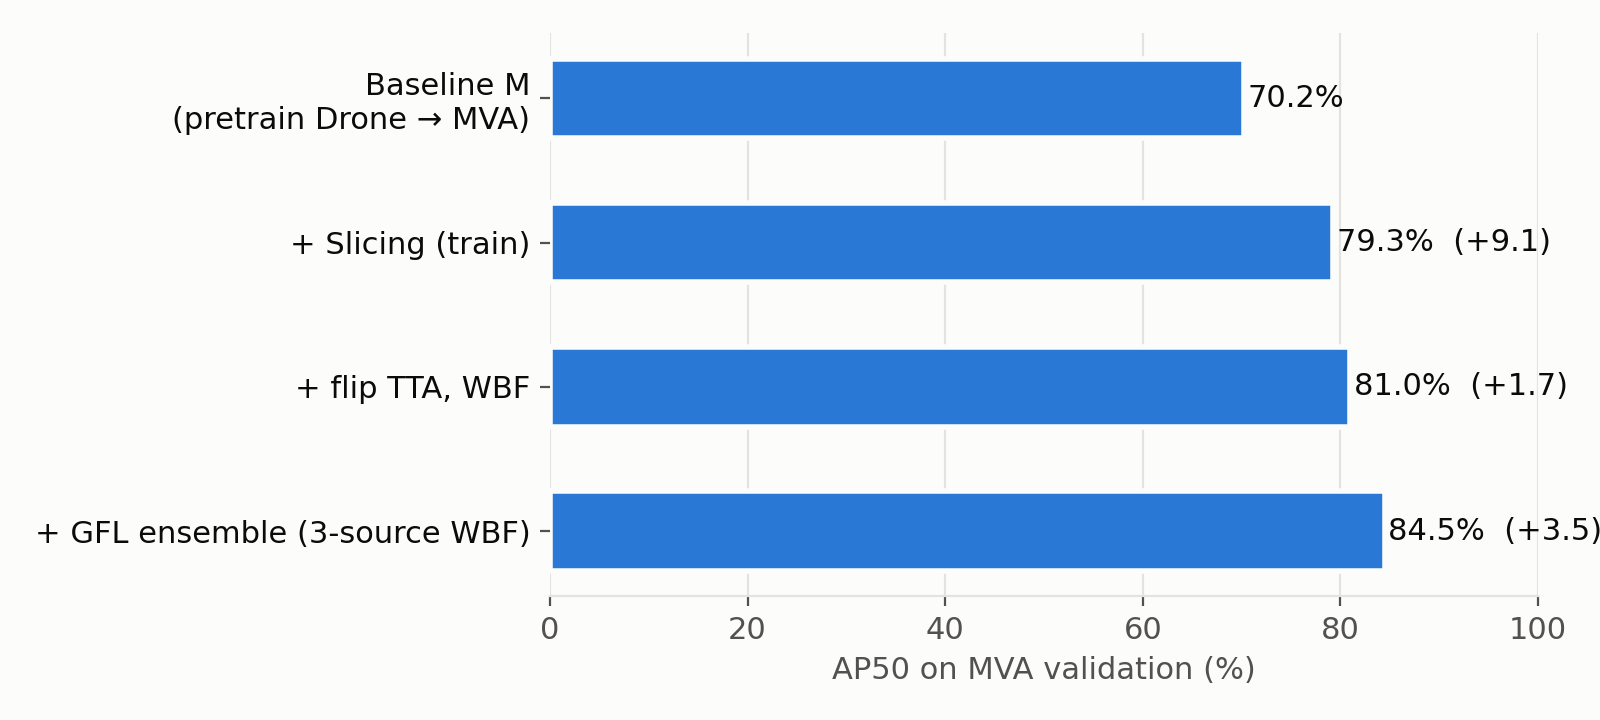
\includegraphics[width=0.75\textwidth]{figures/01_pipeline_progression.png}
\caption{AP50 after each step of the final pipeline.}
\label{fig:progress}
\end{figure}

\subsection{Further Analysis}
This section examines each design choice in turn.

\subsubsection{Training-Time Ablation}
Table~\ref{tab:train} compares the data strategies. Colour augmentation does not help ($-0.2$): the frames already
span a wide range of illumination. Copy-paste hurts ($-3.3$), presumably because pasted patches have inconsistent
blur, lighting and context with the target background, which teaches the detector shortcuts that do not transfer.
Slicing improves every metric, most strongly AP75 (+13.3); note that it also uses 3.6 times more samples per epoch (Section~\ref{sec:limits}).

\begin{table}[t]
\caption{Training-time strategies (YOLOv8-M, 30 epochs, \%).}
\label{tab:train}
\centering
\setlength{\tabcolsep}{4pt}
\begin{tabular}{lccc}
\toprule
Strategy & AP50 & AP75 & AR100 \\
\midrule
YOLOv8-M baseline & 70.2 & 25.5 & 43.9 \\
\quad + colour aug. & 70.0 & 25.5 & 43.8 \\
\quad + copy-paste & 66.9 & 23.2 & 42.2 \\
\quad + slicing & \textbf{79.3} & \textbf{38.8} & \textbf{50.0} \\
\midrule
Drone2021 pretrain only & 0.1 & 0.0 & 2.5 \\
\bottomrule
\end{tabular}
\end{table}

\textbf{Pretraining alone.} The Drone2021 model scores 0.1\% AP50 on MVA without fine-tuning, yet its most confident
false positives lie on real birds (Fig.~\ref{fig:pretrain}): its boxes are much larger than the MVA annotations
(median $\sqrt{\text{area}}$ of 40 px for predictions with score above 0.3, against 16 px for MVA boxes and 25--31 px for
Drone2021 boxes). Fine-tuning therefore mainly adapts the box convention, not the notion of a bird.

\begin{figure}[t]
\centering
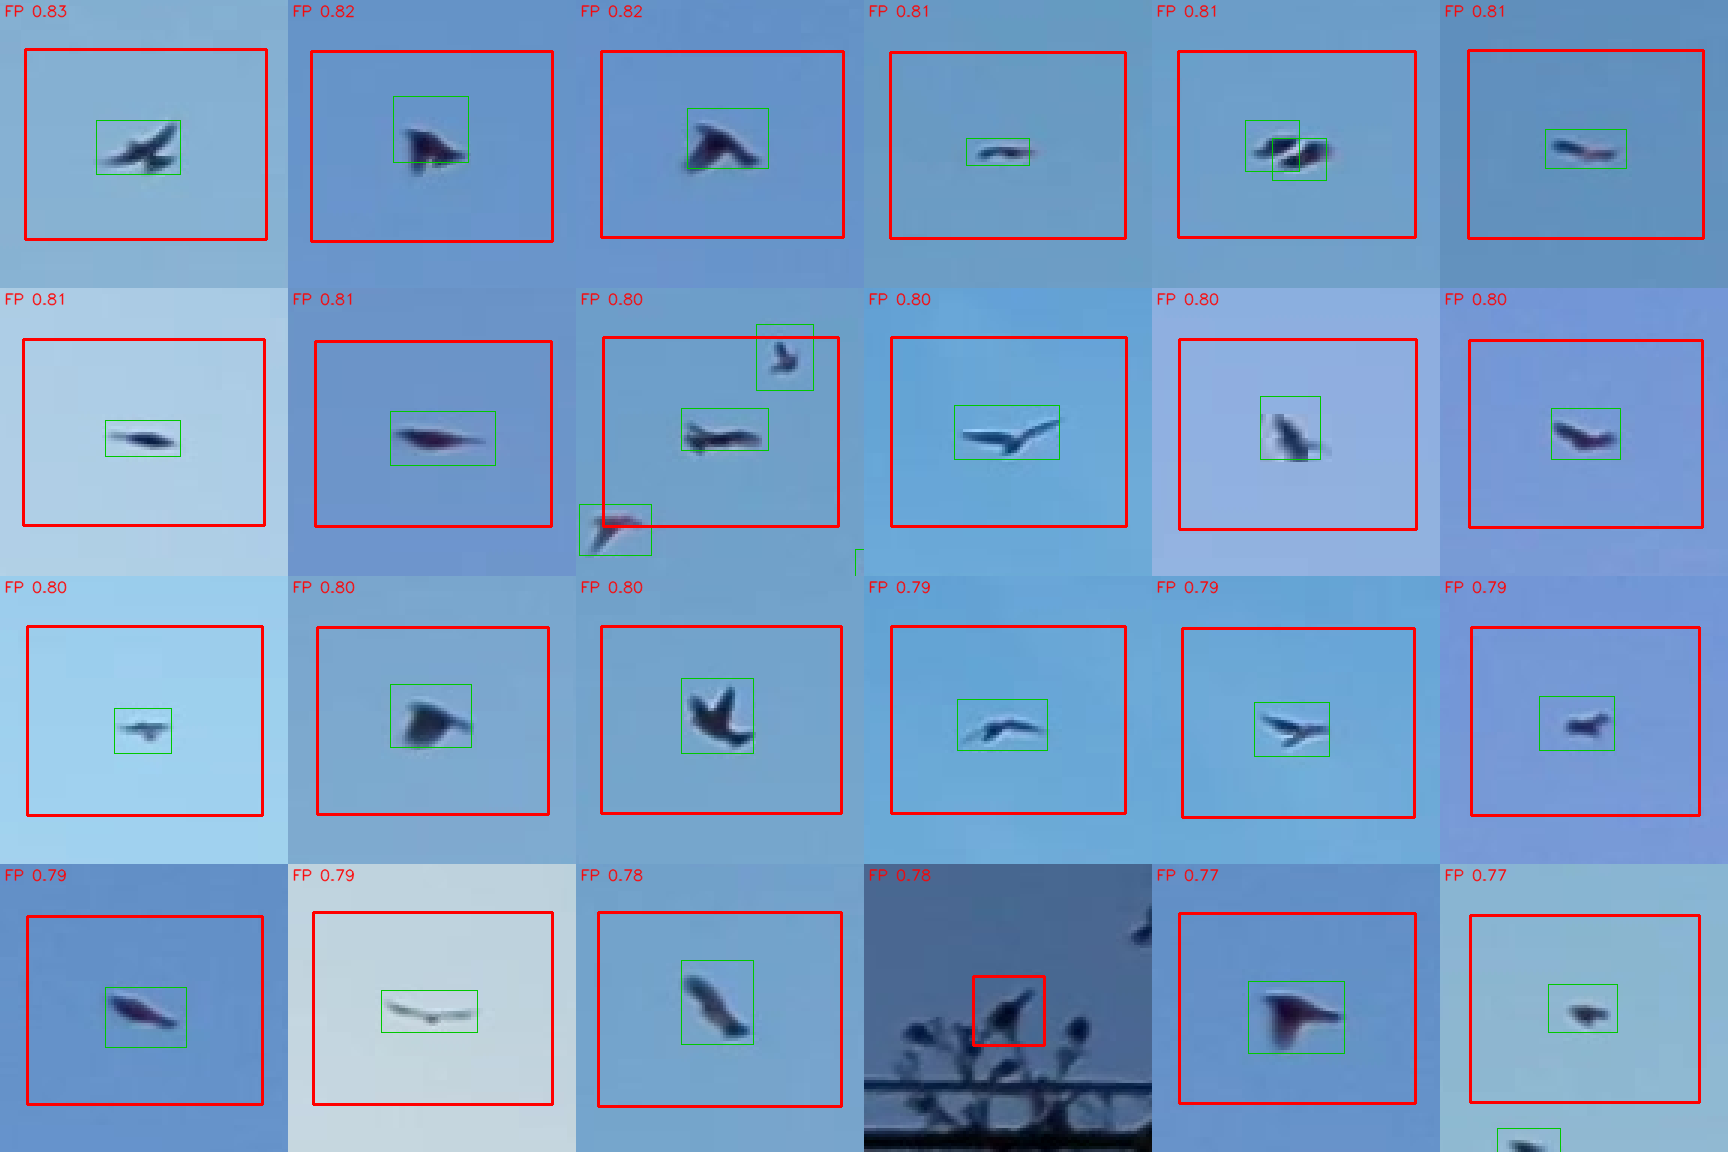
\includegraphics[width=0.75\textwidth]{figures/04_pretrain_only_fp.png}
\caption{Most confident false positives of the Drone2021-only model on MVA (red: prediction, green: ground truth).
The birds are found, but the boxes are too large to reach IoU 0.5.}
\label{fig:pretrain}
\end{figure}

\subsubsection{Inference-Time Ablation and the Failure of SAHI}
Table~\ref{tab:infer} reports inference variants on the slicing model. Flip TTA gives a small, consistent gain. SAHI
with $z=1.5$ loses 11.8 AP50 under NMS, and AP75 drops far more (38.8\% to 28.7\%) than AR100 (50.0\% to 47.4\%):
the birds are still found, but many of their boxes become imprecise. Three mechanisms explain the loss. First, \emph{no information is added}:
the full frame is already processed at native resolution, so a zoomed tile only interpolates existing pixels.
Second, \emph{scale mismatch}: zooming by 1.5 turns 32--64 px birds into 48--96 px birds, a size rarely seen in
training. Third, \emph{tile artefacts}: birds cut by a tile border produce partial boxes with low IoU to the
full-frame box, which NMS does not suppress, and bird-free tiles produce confident false positives (at the best F1
operating point, false positives rise from 224 to 786). Discarding border-touching boxes and halving tile scores
recover 10.2 points; with $z=1$ the tiles match the training distribution and SAHI reaches, but does not exceed,
plain inference while being three times slower.

\begin{table}[t]
\caption{Inference variants of the slicing model (\%). ``Fixed'' is the best correction of Section~\ref{sec:inference};
tiles per frame in brackets.}
\label{tab:infer}
\centering
\setlength{\tabcolsep}{3pt}
\begin{tabular}{llcccr}
\toprule
Inference & Merge & AP50 & AP75 & AR100 & ms \\
\midrule
Full frame & -- & 79.3 & 38.8 & 50.0 & 337 \\
Flip TTA & NMS 0.6 & 79.9 & 38.5 & 50.6 & 709 \\
 & WBF & \textbf{81.0} & \textbf{40.3} & \textbf{51.1} & 709 \\
SAHI, $z=1.5$ (36) & NMS 0.6 & 67.5 & 28.7 & 47.4 & 1748 \\
 & fixed & 77.7 & 38.3 & 49.3 & 1748 \\
SAHI, $z=1.5$ + flip (72) & NMS 0.6 & 66.0 & 27.5 & 47.9 & 3621 \\
 & fixed & 78.2 & 38.0 & 49.6 & 3621 \\
SAHI, $z=1.0$ (16) & NMS 0.6 & 78.5 & 38.0 & 50.2 & 963 \\
 & fixed & 79.3 & 38.6 & 49.5 & 963 \\
\bottomrule
\end{tabular}
\end{table}

\subsubsection{Fusion Strategies}
Table~\ref{tab:fusion} compares ways of combining the two YOLO views with GFL. All three reach 84.4--84.5\% AP50; the
one-stage fusion has the best AP75 and AR100 and needs no tuned weights, so it is used for the submission. Its held-out
check confirms the gain: choosing the rule on one half of the validation set and scoring the other gives 84.1\% and
84.8\%, against 80.7\% and 81.4\% for flip TTA alone.

\begin{table}[t]
\caption{Fusion of YOLO (plain + flip) and GFL (\%).}
\label{tab:fusion}
\centering
\setlength{\tabcolsep}{3.5pt}
\begin{tabular}{lccc}
\toprule
Fusion & AP50 & AP75 & AR100 \\
\midrule
TTA by NMS $\rightarrow$ WBF with GFL & 84.4 & 45.2 & 52.9 \\
TTA by WBF $\rightarrow$ WBF, $w_{\text{YOLO}}{=}1.5$ & 84.5 & 45.3 & 53.3 \\
One-stage WBF, 1:1:1 & \textbf{84.5} & \textbf{45.8} & \textbf{53.4} \\
\bottomrule
\end{tabular}
\end{table}

\subsubsection{Why the Ensemble Works: Scale-Wise Analysis}
Table~\ref{tab:scale} and Fig.~\ref{fig:scale} split AP50 by bird size. YOLO is clearly better on 8--16 px birds
(80.2\% vs.\ 67.4\%), which make up half of the validation set; a likely reason is that YOLO sees them at native
resolution, whereas GFL works on a frame downscaled to 2/3. GFL is clearly better on 32--64 px birds (72.4\% vs.\
60.6\%); we hypothesise that the downscaled input gives each feature more context, which helps against the
camouflage that dominates errors at this size (Section~\ref{sec:errors}), but we have not isolated this effect. The ensemble inherits the stronger model in each bucket and reduces
false negatives from 698 to 611 at the best F1 operating point.

\begin{table}[t]
\caption{AP50 (\%) by $\sqrt{\text{area}}$, overall AR100 (\%) and best-F1 operating point. Buckets with fewer
than 20 birds are omitted.}
\label{tab:scale}
\centering
\footnotesize
\setlength{\tabcolsep}{2pt}
\begin{tabular}{lcccccc}
\toprule
Model & 8--16 & 16--32 & 32--64 & AR100 & F1 & FP/FN \\
 & (1{,}456) & (1{,}070) & (316) & & & \\
\midrule
YOLO baseline & 64.3 & 80.3 & 58.9 & 43.9 & 71.8 & 495/984 \\
YOLO slicing & 78.4 & 86.1 & 58.4 & 50.0 & 81.8 & 224/728 \\
YOLO slic.\ + TTA & 80.2 & 87.6 & 60.6 & 51.1 & 82.9 & 198/698 \\
GFL & 67.4 & 87.7 & \textbf{72.4} & 46.6 & 77.4 & 216/920 \\
Ensemble & \textbf{83.5} & \textbf{89.4} & \textbf{72.4} & \textbf{53.4} & \textbf{84.5} & 218/\textbf{611} \\
\bottomrule
\end{tabular}
\end{table}

\begin{figure}[t]
\centering
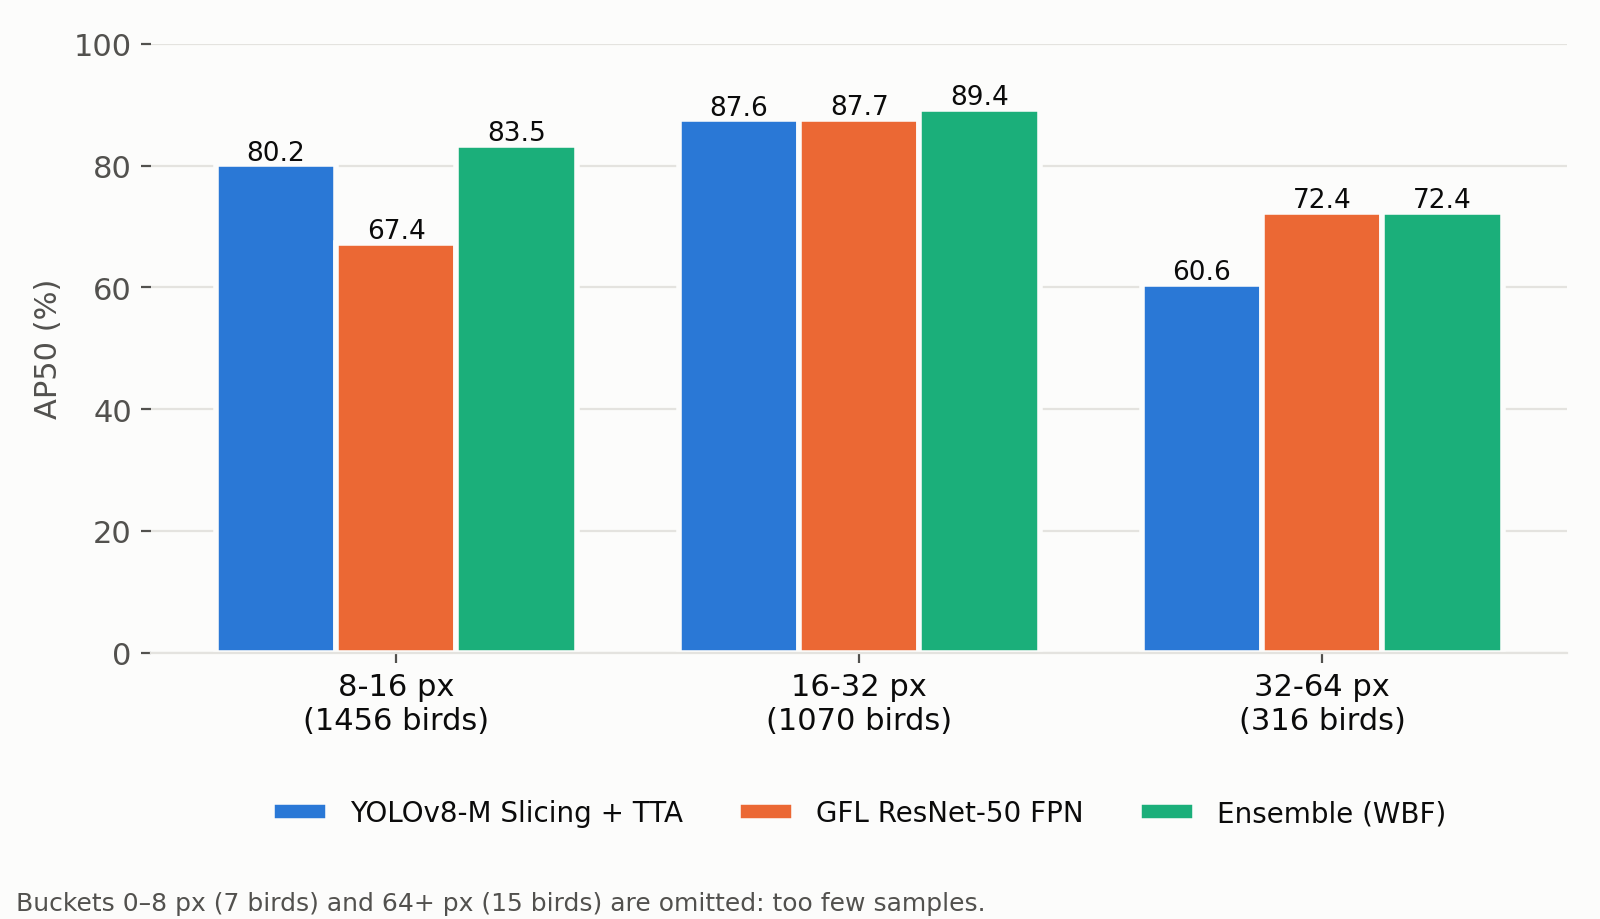
\includegraphics[width=0.75\textwidth]{figures/02_ap50_by_size.png}
\caption{AP50 by bird size. YOLO and GFL are strong on different sizes; the ensemble keeps the better of the two.}
\label{fig:scale}
\end{figure}

\subsubsection{Remaining Errors}
\label{sec:errors}
Fig.~\ref{fig:fn} shows false negatives of the YOLO model. Most misses are birds camouflaged in grass or foliage,
birds on wires and poles, and birds against dark or over-exposed backgrounds; a few are barely visible even to a
human annotator. These are failures of appearance rather than of resolution, which is consistent with the
plateau of the 32--64 px bucket across all YOLO variants.

\begin{figure}[t]
\centering
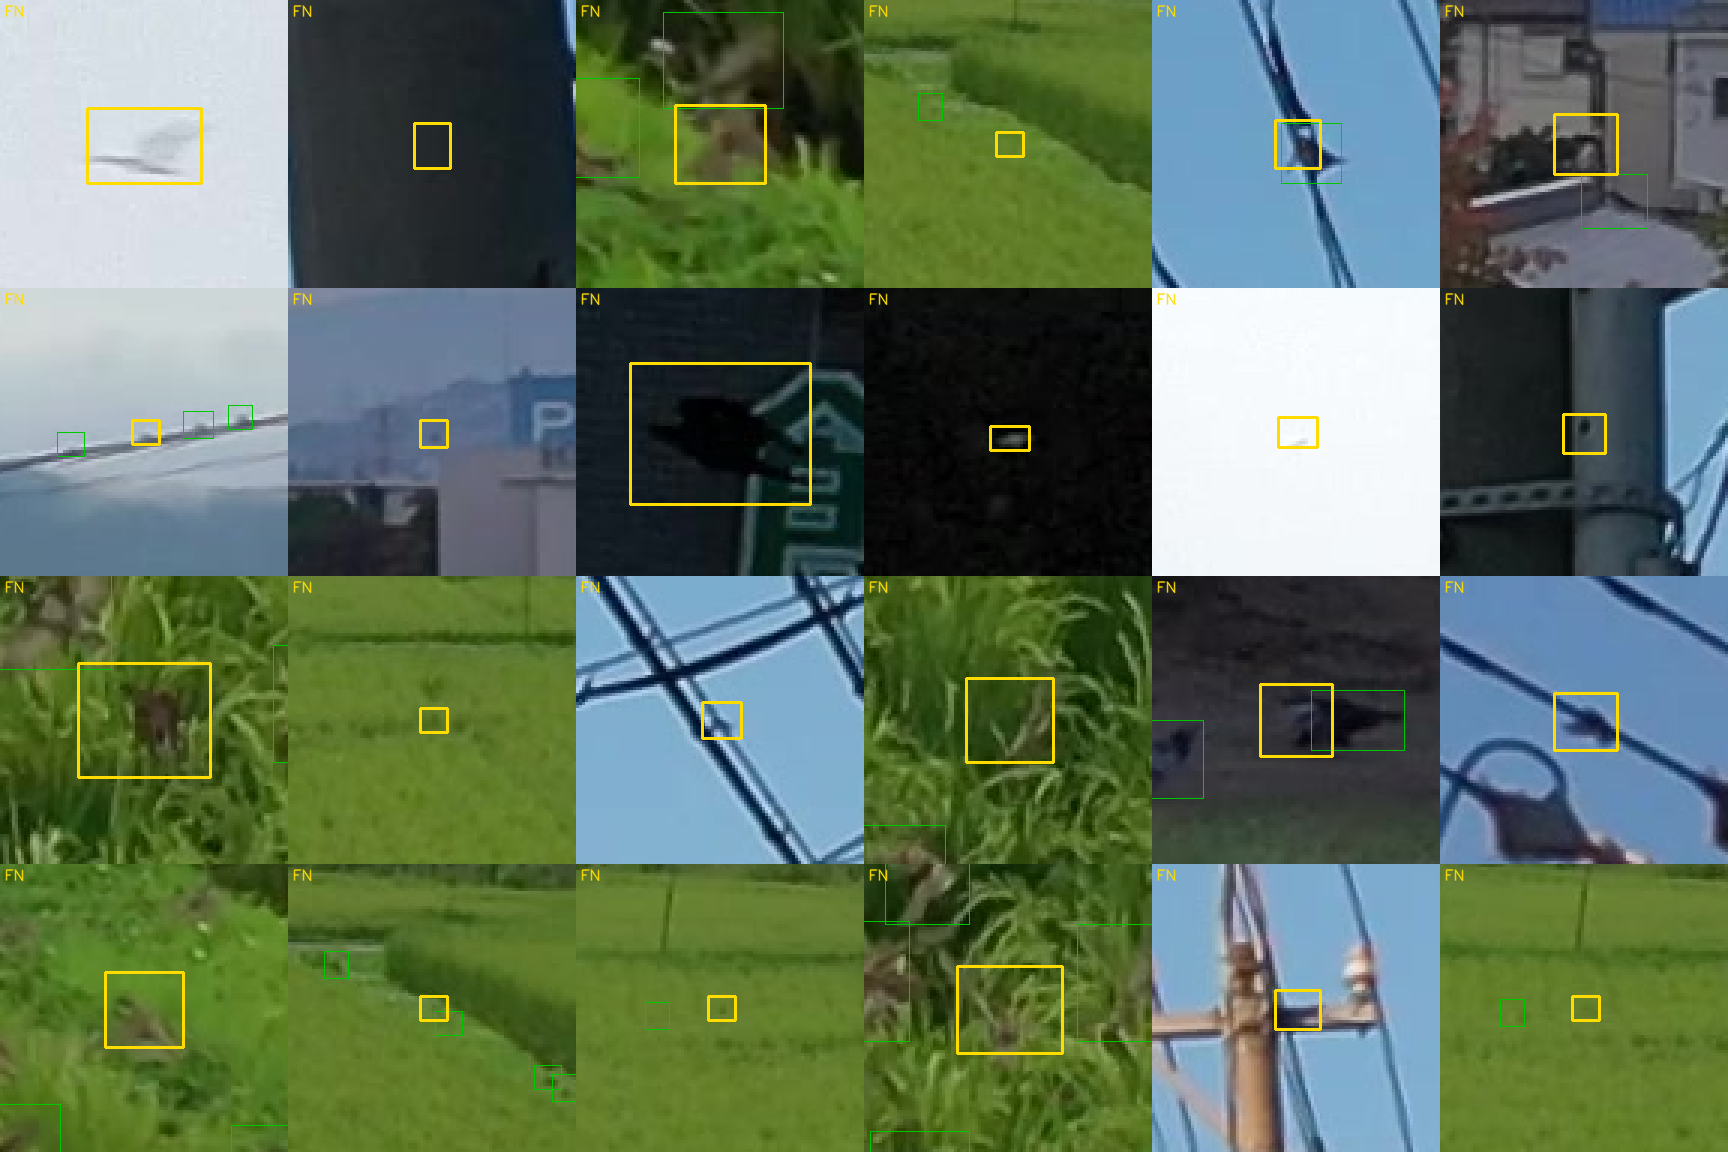
\includegraphics[width=0.75\textwidth]{figures/03_false_negatives.png}
\caption{False negatives of YOLO slicing + TTA (yellow: missed bird, green: other annotated birds). Crops are
96$\times$96 px enlarged three times.}
\label{fig:fn}
\end{figure}

\subsection{Limitations}
\label{sec:limits}
First, slicing changes two factors at once: it covers every bird in every epoch and it produces 3.6 times more
samples, hence more optimiser updates, than the other branches. Our ablation does not separate the two; a
compute-matched baseline is left for future work. Second, all comparisons use a single seed, and the GFL checkpoint was chosen on the validation set (about 0.7 AP50
above its last epoch), which slightly favours GFL and the ensemble. Third, validation
frames come from the same videos as training frames, so scene-level generalisation is not measured, and the public
test score was not available to us at the time of writing.

%=====================================================================
\section{Development Process and Practical Challenges}
\label{sec:process}
%=====================================================================
The project ran for about seven weeks, from mid-September to 6 November 2026, on a single laptop GPU (RTX 5070 Laptop,
8~GB, Blackwell architecture). Table~\ref{tab:timeline} summarises the phases. This section reports the route that led
to the final system, including the branches that were abandoned, because several of the design choices of
Section~\ref{sec:method} were forced by these constraints rather than chosen freely.

\begin{table}[t]
\caption{Project timeline (2026). AP50 on the validation split of the dataset named in each row.}
\label{tab:timeline}
\centering
\footnotesize
\setlength{\tabcolsep}{2.5pt}
\begin{tabular}{l>{\raggedright\arraybackslash}p{4.1cm}>{\raggedright\arraybackslash}p{1.7cm}}
\toprule
Period & Work & Outcome \\
\midrule
16--27 Sep & GPU environment; released GFL checkpoint re-evaluated; GFL from scratch on MVA only & 88.9\% (released); 6.1\% after 1 epoch \\
27 Sep--7 Oct & GFL: Drone2021 6 epochs, then MVA 50 epochs with per-image BN & 74.9\% (MVA) \\
9--28 Oct & First round of YOLO and Swin experiments (batch of one); discarded on 29 Oct & not used \\
29--31 Oct & YOLOv8-S on Drone2021: BN failure diagnosed, crop recipe rewritten & 47.4\% (Drone) \\
31 Oct--1 Nov & YOLOv8-S on MVA (colour augmentation); switch to the M model & 68.8\% (MVA) \\
1--2 Nov & YOLOv8-M on Drone2021, 10 epochs (Drone2021 re-downloaded) & 44.6\% (Drone) \\
2--4 Nov & YOLOv8-M: baseline and three data strategies, 30 epochs each & 66.9--79.3\% (MVA) \\
4 Nov & TTA, SAHI, merging rules, GFL ensemble, error analysis & 84.5\% (MVA) \\
4--5 Nov & Public-test inference (9{,}699 frames) & submission file \\
5--6 Nov & Paper, code and weight release & -- \\
\bottomrule
\end{tabular}
\end{table}

\subsection{Pipeline Verification}
Before any training, the inference and evaluation code was checked against a published number. The GFL checkpoint
released with the challenge baseline~\cite{kondo2023sod4sb,shinya2022usb}, which is initialised from COCO-pretrained
weights and processes full 3840$\times$2160 frames, reproduces its reported 47.0\% AP and 88.9\% AP50 (with flip TTA) on the same
879 validation frames with our code. Our own models are trained without any downloaded weights, a constraint fixed at the
start of the project; this explains most of the gap to that reference and is the main reason our numbers should not be
compared with challenge entries. A GFL trained from scratch on MVA alone reached only 6.1\% AP50 after one epoch, which
led us to pretrain both detectors on Drone2021.

\subsection{Challenges and How They Were Addressed}
\textbf{A new GPU with old libraries.} The Blackwell GPU (compute capability 12.0) requires PyTorch 2.7 with CUDA 12.8,
for which no binary build of MMCV~1.6, the basis of the GFL code, exists. We used the pure-Python MMCV with a small
compatibility layer that replaces its CUDA operators by torchvision NMS, and verified it on six NMS test cases of 1{,}200
boxes against the original CPU implementation (identical outputs); on two test frames GPU inference was about 19 times faster
than the CPU fallback. Data-loader worker processes hung on Windows and were disabled for GFL inference.

\textbf{BatchNorm with a batch of one.} Fitting 2560$\times$1440 inputs into 8~GB forced a physical batch of one with
gradient accumulation. Batch normalisation then normalises each image with its own statistics during training but uses
running averages at test time. For GFL this was fixed by using per-image normalisation in both training and inference.
The first YOLO pretraining run suffered from the same mismatch without it being visible in the loss: its validation
AP50 fell to 3.4\% at epoch~4, while re-evaluating the same weights with per-image statistics on 500 frames gave
35--37\%. We
therefore rewrote the YOLO recipe to train on native-resolution 1280$\times$736 crops with real batches (8 for
YOLOv8-S, 6 for YOLOv8-M), which is also how slicing entered the study. For YOLOv8-M a batch of 8 filled the GPU memory
and ran at 14.3 images/s; a batch of 6 ran at 18.6 images/s. Mixed-precision overflow occurred 37 times during GFL
training (10 on Drone2021, 27 on MVA); each time the step was retried with a halved loss scale.

\textbf{Throughput and reliability of a laptop.} Decoding 4K JPEG frames limited YOLO training to 12.3 images/s;
decoding and crop generation in a thread pool raised this to 25.8 images/s. After a restart, Windows power management
moved the data-loading threads to efficiency cores and throughput fell to about 10 images/s, until a wrapper disabled
power throttling for the training process. Training was interrupted by a GPU driver reset, by an application-hang
termination during validation and by planned shutdowns. All trainers therefore save atomic checkpoints (model,
optimiser, scaler, random-number state and position in the epoch), and resumption was verified to give exactly the
same result as uninterrupted training; the hash of the training code is stored with each run, so that a resumed run
cannot silently use modified code. Public-test inference was first stopped after about 3{,}700 of 9{,}699 frames and
lost; it was rewritten to save results in chunks of 500 frames.

\textbf{Data.} One exactly duplicated box was removed from the validation labels. Drone2021 and MVA use different box
conventions (Section~\ref{sec:experiments}), and Drone2021 pretraining overfitted after 4 epochs for YOLOv8-S and 7
for YOLOv8-M; a second pretraining phase with stronger augmentation did not improve the starting point and was not
used. Most misses of 32--64~px birds by YOLOv8-S came from three frames with dense flocks (124 of 134 misses). The 63.5~GB of
Drone2021 images had to be deleted for disk space and downloaded again when we moved from YOLOv8-S to YOLOv8-M.

\textbf{Compute budget and abandoned branches.} With one GPU every experiment delayed the next, so the plan changed
several times. A first round of YOLO and Swin Transformer experiments (9--28 October; native and upscaled crops,
NWD loss, DySample upsampling) had been run with a batch of one; on 29 October it was discarded and the YOLO study
was restarted under one controlled protocol, so none of its results are used here. YOLOv8-S was stopped after one MVA strategy in favour of YOLOv8-M. A YOLOv8-M variant with an additional
high-resolution P2 head and a combined recipe (slicing, copy-paste and colour augmentation in one run) were prepared and
tested on the CPU; the combined recipe was started on free cloud T4 GPUs, but both were dropped to meet the deadline.
Instead, the remaining time went into inference-time methods and the heterogeneous ensemble, which need no further
training. A missing plain YOLOv8-M baseline was noticed late and trained before the ablation was considered complete.

\subsection{Lessons}
Three lessons transfer to similar projects. First, verify the evaluation code against a published checkpoint before
training anything. Second, with small batches, check batch normalisation explicitly: a train/test mismatch can look
like overfitting. Third, on a single consumer GPU, resumable training with verified exact resumption and pinned code is
worth its cost, because interruptions are the rule rather than the exception.

%=====================================================================
\section{Conclusion}
%=====================================================================
We studied where resolution should be preserved for detecting tiny birds in 4K frames. Exhaustive native-resolution
tile sampling during training is the most effective single change. Tiled inference with SAHI is redundant, and
harmful, once frames are processed without downscaling; its loss is explained by scale mismatch and tile artefacts.
Flip TTA merged with WBF and a heterogeneous WBF ensemble with GFL are complementary, raising AP50 from 70.2\% to
84.5\%, AP75 from 25.5\% to 45.8\% and AR100 from 43.9\% to 53.4\%, because the two detectors are strong on different bird sizes. Future work will separate the effects of tile
coverage and update count in slicing, and target camouflaged birds, which dominate the remaining errors.

\backmatter

\bmhead{Supplementary information}
Per-image predictions, per-epoch metrics and every result table are provided in the code repository
(Code availability).

\section*{Declarations}

\begin{itemize}
\item \textbf{Funding:} [to be completed by the authors].
\item \textbf{Conflict of interest/Competing interests:} The authors declare that they have no known competing
financial interests or personal relationships that could have appeared to influence the work reported in this paper.
\item \textbf{Ethics approval and consent to participate:} Not applicable.
\item \textbf{Consent for publication:} Not applicable.
\item \textbf{Data availability:} The MVA 2023 SOD4SB and Drone2021 images are not redistributed and can be obtained
from the challenge organisers; the audited label manifest is included in the code repository.
\item \textbf{Materials availability:} Not applicable.
\item \textbf{Code availability:} Code, configurations, per-image results and trained weights are available at
\url{https://github.com/sotbatchien123/sod4sb-small-bird-detection}.
\item \textbf{Author contribution:} [to be completed by the authors].
\end{itemize}

\bibliography{refs}

\end{document}
